\chapter{Функции обработчика прерывания от системного таймера}

\section{Windows}

\subsection{По тику}
\begin{enumerate}
	\item Инкремент счётчика системного времени;
	\item Декремент кванта текущего потока на величину, равную количеству тактов процессора,произошедших за тик. В случае, если количество затраченных потомков тактов процессора достигает квантовой цели, запускается обработка истечения кванта;
	\item Декремент счетчиков времени отложенных задач;
	\item В случае, если активен механизм профилирования ядра, инициализирует отложенный вызов обработчика ловушки профилирования ядра путём постановки объекта в очередь DPC: обработчик ловушки профилирования регистрирует адрес команды, выполнявшейся на момент прерывания.
\end{enumerate}

\subsection{По главному тику}
\begin{enumerate}
	\item Инициализация диспетчера настройки баланса путем сбрасывания объекта «событие», на котором он ожидает.
\end{enumerate}

\subsection{По кванту}
\begin{enumerate}
	\item Инициализация диспетчеризации потоков – постановка соответствующего объекта в очередь DPC.
\end{enumerate}

\section{Unix}

\subsection{По тику}
\begin{enumerate}
	\item Инкремент счётчика тиков аппаратного таймера;
	\item Декремент кванта текущего потока;
	\item Обновление статистики использования процессора текущим процессом – инкремент поля c\_cpu дескриптора текущего процесса до максимального значения 127;
	\item Инкремент часов и других таймеров системы;
	\item Декремент счетчика времени до отправления на выполнение отложенных вызовов, при достижении счетчиком нуля выставление флага для обработчика отложенных вызовов.
\end{enumerate}

\subsection{По главному тику}
\begin{enumerate}
	\item Регистрация отложенных вызовов функций, относящихся к работе планировщика;
	\item Регистрация отложенных вызовов процедуры wakeup, которая перемещает дескрипторы процессов из очереди «спящих» в очередь «готовых к выполнению»;
	\item Декремент счетчика времени, оставшегося до отправления одного из сигналов:
	\begin{itemize}
		\item SIGALARM - сигнал, посылаемый процессу по истечении времени;
		\item SIGPROF - сигнал, посылаемый процессу по истечении времени заданном в таймере профилирования;
		\item SIGVTALARM - сигнал, посылаемый процессу по истечении времени, заданного
		в «виртуальном» таймере.
	\end{itemize}
\end{enumerate}

\subsection{По кванту}
\begin{enumerate}
	\item Отправка сигнала SIGXCPU текущему процессу, если тот превысил выделенную для него квоту использования процессора.
\end{enumerate}

\chapter{Пересчет динамических приоритетов}

Динамическими приоритетами являются приоритеты пользовательских процессов. 
В отчете пересчет динамических приоритетов рассматривается отдельно для ОС семейства Windows и для ОС Unix.

\section{Windows}

В Windows при создании процесса, ему назначается базовый приоритет. Относительно
базового приоритета процесса потоку назначается относительный приоритет.

Планирование осуществляется на основании приоритетов потоков, готовых к выполнению. В Windows поток с более низким приоритетом вытесняется планировщиком, когда поток с более высоким приоритетом становится готовым к выполнению. Диспетчер настройки
баланса сканирует очередь готовых потоков раз в секунду и, если обнаружены потоки, ожидающие выполнения более 4 секунд, диспетчер настройки баланса повышает их приоритет
до 15 единиц и устанавливает квантовую цель эквивалентной тактовой частоте процессора
при подсчете 3 квантовых единиц. Как только квант истекает, приоритет потока снижается
до базового приоритета. Если поток не был завершен за квант времени или был вытеснен
потоком с более высоким приоритетом, то после снижения приоритета поток возвращается в
очередь готовых потоков. Диспетчер настройки баланса сканирует лишь 16 готовых потоков
и повышает приоритет не более чем у 10 потоков за один проход. При следующем проходе
сканирование возобновляется с того места, где оно было прервано в прошлый раз. Наличие 10 потоков, приоритет которых следует повысить, свидетельствует о необычно высокой
загруженности системы.

\newpage
Windows использует 32 уровня приоритета, от 0 до 31. Эти значения разбиваются на части следующим образом:
\begin{itemize}
	\item шестнадцать уровней реального времени (от 16 до 31);
	\item шестнадцать изменяющихся уровней (от 0 до 15), из которых уровень 0 зарезервирован
	для потока обнуления страниц.
\end{itemize}

Уровни приоритета потоков назначаются исходя из двух разных позиций: одной от Windows
API и другой от ядра Windows. Сначала Windows API систематизирует процессы по классу
приоритета, который им присваивается при создании: Реального времени — Real-time (4),
Высокий — High (3), Выше обычного — Above Normal (7), Обычный — Normal (2), Ниже
обычного — Below Normal (5) и Простоя — Idle (1). 

Затем назначается относительный приоритет отдельных потоков внутри этих процессов.
Здесь номера представляют изменение приоритета, применяющееся к базовому приоритету
процесса: Критичный по времени — Time-critical (15), Наивысший — Highest (2), Выше обычного — Above-normal (1), Обычный — Normal (0), Ниже обычного — Below-normal (–1), Самый низший — Lowest (–2) и Простоя — Idle (–15).

Исходный базовый приоритет потока наследуется от базового приоритета процесса. Процесс по умолчанию наследует свой базовый приоритет у того процесса, который его создал.
Соответствие между приоритетами Windows API и ядра системы приведено на рисунке 2.1.
\begin{figure}[H]
	\begin{center}
		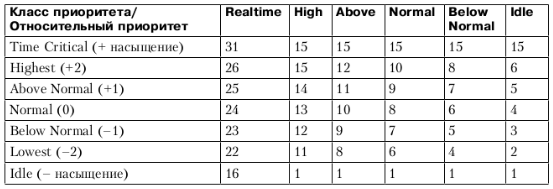
\includegraphics[scale=0.6]{assets/win_pr.png}
	\end{center}
	\caption{Соответствие между приоритетами Windows API и ядра Windows}
\end{figure}

Текущий приоритет потока в динамическом диапазоне — от 1 до 15 — может быть повышен
планировщиком вследствие следующих причин:
\begin{enumerate}
	\item \textbf{Повышение вследствие события планировщика или диспетчера (сокращение
	задержек).} При наступлении события диспетчера вызываются процедуры с целью проверить не должны ли на локальном процессоре быть намечены какие-либо потоки, которые не должны быть спланированы.
	\item \textbf{Повышение приоритета владельца блокировки.} Поскольку блокировки ресурсов
	исполняющей системы (ERESOURCE) и блокировки критических разделов используют основные объекты диспетчеризации, в результате освобождения этих блокировок
	осуществляются повышения приоритета, связанные с завершением ожидания. С другой стороны, поскольку высокоуровневые реализации этих объектов отслеживают владельца блокировки, ядро может принять более взвешенное решение о том, какого вида
	повышение должно быть применено с помощью AdjustBoost.
	\item \textbf{Повышение приоритета после завершения ввода/вывода (сокращение задержек)} (рисунок 2.2). Windows дает временное повышение приоритета при завершении
	определенных операций ввода-вывода, при этом потоки, ожидавшие ввода-вывода, имеют больше шансов сразу же запуститься и обработать то, чего они ожидали.
	\begin{figure}[H]
		\begin{center}
			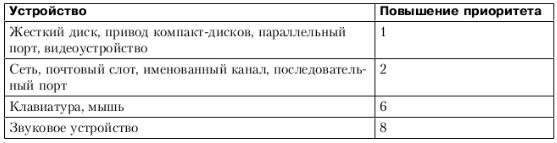
\includegraphics[scale=0.7]{assets/rec_pr.png}
		\end{center}
		\caption{Рекомендуемые значения повышения приоритета}
	\end{figure}
	\item \textbf{Повышение приоритета вследствие длительного ожидания ресурса исполняющей системы(предотвращение зависания).} Когда поток пытается получить
	ресурс исполняющей системы (ERE-SOURCE), который уже находится в исключительном владении другого потока, он должен войти в состояние ожидания до тех пор, пока
	другой поток не освободит ресурс. Для ограничения риска взаимных исключений исполняющая система выполняет это ожидание, не входя в бесконечное ожидание ресурса,
	а интервалами по пять секунд. Если по окончании этих пяти секунд ресурс все еще
	находится во владении, исполняющая система пытается предотвратить зависание центрального процессора путем завладения блокировкой диспетчера, повышения приоритета потока или потоков, владеющих ресурсом, до значения 14 (если исходный приоритет
	владельца был меньше, чем у ожидающего, и не был равен 14), перезапуска их квантов
	и выполнения еще одного ожидания.
	\item \textbf{Повышение приоритета, связанные с завершением ожидания.} Повышения приоритета, связанные с завершением ожидания (unwait boosts), пытаются уменьшить время задержки между потоком, пробуждающимся по сигналу объекта (переходя тем самым в состояние Ready), и потоком, фактически приступившим к своему выполнению в
	процессе, который не находился в состоянии ожидания (переходя тем самым в состояние
	Running).
	\item \textbf{Повышение приоритета после пробуждения GUI-потока.} Потоки - владельцы окон
	получают при пробуждении дополнительное повышение приоритета на 2 из-за активности системы работы с окнами, например поступление сообщений от окна. Система
	работы с окнами (Win32k.sys) применяет это повышение приоритета, когда вызывает
	функцию KeSetEvent для установки события, используемого для пробуждения GUI-
	потока. Смысл этого повышения похож на смысл предыдущего повышения — содействие
	интерактивным приложениям.
	\item \textbf{Повышения приоритета, связанные с перезагруженностью центрального процессора.} В Windows также включен общий механизм ослабления загруженности центрального процессора, который называется диспетчером настройки баланса и является частью потока (речь идет о системном потоке, который существует главным образом для выполнения функций управления памятью). Один раз в секунду этот поток сканирует очередь готовых потоков в поиске тех из них, которые находятся в состоянии ожидания (то есть не были запущены) около 4 секунд. Если такой поток будет найден, диспетчер настройки баланса повышает его приоритет до 15 единиц и устанавливает квантовую цель эквивалентной тактовой частоте процессора при подсчете 3 квантовых единиц. Как только квант истекает, приоритет потока тут же снижается до обычного базового приоритета. Если поток не был завершен и есть готовый к запуску поток с
	более высоким уровнем приоритета, поток с пониженным приоритетом возвращается в
	очередь готовых потоков, где он опять становится подходящим для еще одного повышения приоритета, если будет оставаться в очереди следующие 4 секунды.
	\item \textbf{Повышение приоритета потоков первого плана после ожидания.} Смысл этого
	повышения заключается в улучшении отзывчивости интерактивных приложений: если
	дать приложениям первого плана небольшое повышение приоритета при завершении
	ожидания, у них повышаются шансы сразу же приступить к работе, особенно когда
	другие процессы с таким же базовым приоритетом могут быть запущены в фоновом
	режиме.
	\item \textbf{Повышение приоритета проигрывания мультимедиа службой планировщика
	MMCSS.}
	Повышение приоритета проигрывания мультимедиа обычно управляется службой пользовательского режима, которая называется службой планировщика класса мультимедиа - MultiMedia Class Scheduler Service (MMCSS). MMCSS работает с вполне определенными задачами, включая следующие: аудио, захват, распределение, игры, проигрывание, аудио профессионального качества, задачи администратора многооконного режима. 
	
	В свою очередь, каждая из этих задач включает информацию о свойствах, отличающих
	их друг от друга. Одно из наиболее важных свойств для планирования потоков называется категорией планирования — Scheduling Category, которое является первичным
	фактором, определяющим приоритет потоков, зарегистрированных с MMCSS.
	Механизм, положенный в основу MMCSS, повышает приоритет потоков внутри зарегистрированного процесса до уровня, соответствующего их категории планирования.
	Затем он снижает категорию этих потоков до Exhausted, чтобы другие, не относящиеся
	к мультимедийным приложениям потоки, также могли получить ресурс.
\end{enumerate}

\section{Unix}

В ОС семейства LINUX и UNIX динамически пересчитываться могут только приоритеты пользовательских процессов. В ОС владельцем ресурсов (в том числе и владельцем
приоритета) является процесс.

В современных системах UNIX ядро является вытесняющим. Вытесняемое ядро означает,
что процесс в режиме ядра может быть вытеснен более приоритетным процессом в режиме
ядра. Это сделано для того, чтобы система могла обслуживать процессы реального времени,
такие как аудио и видео.

Приоритет задается любым целым числом, лежащим в диапазоне от 0 до 127. Чем меньше
такое число, тем выше приоритет. Приоритеты от 0 до 49 зарезервированы для ядра, они а
являются фиксированными величинами Прикладные процессы могут обладать приоритетом
в диапазоне 50-127. В первую очередь выполняются процессы с большим приоритетом, а
2процессы с одинаковыми приоритетами выполняются в течении кванта времени циклически
друг за другом. На рисунке 2.3 приведены поля структуры рrос, относящиеся к приоритетам.

\begin{figure}[H]
	\begin{center}
		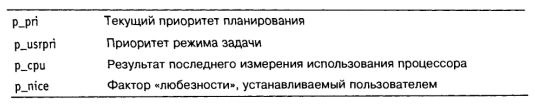
\includegraphics[scale=0.6]{assets/pr.png}
	\end{center}
	\caption{Поля структуры рrос, относящиеся к приоритетам}
\end{figure}

Планировщик использует p\_pri для принятия решения о том, какой процесс направить на
выполнение. У процесса, находящегося в режиме задачи, значения p\_pri и p\_usrpri идентичны. Значение текущего приоритета p\_pri может быть повышено планировщиком для выполнения процесса в режиме ядра. В этом случае p\_usrpri будет использоваться для хранения приоритета, который будет назначен процессу при возврате в режим задачи. Приоритет в
режиме задачи зависит от двух факторов:
\begin{itemize}
	\item фактор любезности;
	\item последней измеренной величины использования процессора.
\end{itemize}

Фактор любезности – целое число в диапазоне от 0 до 39 со значением 20 по умолчанию.
Увеличение фактора любезности приводит к уменьшению приоритета процесса. Фактор любезности процесса может быть изменен суперпользователем с помощью системного вызова
nice.
Системы разделения времени пытаются выделить процессорное время таким образом, что-
бы конкурирующие процессы получили его примерно в равных количествах. Такой подход
требует слежения за использованием процессора каждым из процессов. При создании процесса поле p\_cpu инициализируется нулем. На каждом тике обработчик таймера увеличивает
поле p\_cpu текущего процесса на единицу, до максимального значения, равного 127.
Ядро системы связывает приоритет сна с событием или ожидаемым ресурсом, из-за которого процесс может блокироваться. Когда процесс просыпается после блокирования в си-
стемном вызове, ядро устанавливает в поле p\_pri приоритет сна – значение приоритета из
диапазона от 0 до 49, зависящее от события или ресурса по которому произошла блокировка.
Поскольку приоритеты ядра выше, чем приоритеты режима задачи, такие процессы будут
назначены на выполнение раньше, чем другие, функционирующие в режиме задачи. Такой
подход позволяет системным вызовам быстро завершать свою работу, что является желательным, так как процессы во время выполнения вывзова могут занимать некоторые ключевые
ресурсы системы, не позволяя пользоваться ими другим. На рисунке 2.4 показано событие и
связанное с ним значение приоритета сна.

\begin{figure}[H]
	\begin{center}
		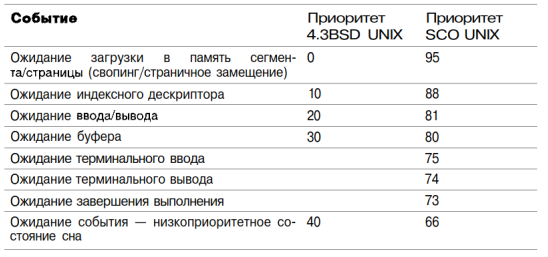
\includegraphics[scale=0.6]{assets/sleep_pr.png}
	\end{center}
	\caption{Системные приоритеты сна}
\end{figure}

Каждую секунду, обработчик прерывания инициализирует отложенный вызов процедуры
schedcpu(), которая уменьшает значение p\_cpu каждого процесса исходя из фактора ”полу-
распада”, который рассчитывается по формуле 2.1, где $load\_average$ - это среднее количество
процессов, находящихся в состоянии готовности к выполнению, за последнюю секунду.
\begin{equation}
	decay = \frac{2 \cdot load\_average}{2\cdot load\_average + 1}
\end{equation}

Процедура schedcpu() пересчитывает приоритеты для режима задачи всех процессов по
формуле 2.2, где PUSER - базовый приоритет в режиме задачи, равный 50.
\begin{equation}
	p\_usrpri = PUSER + \frac{p\_cpu}{2} +  2 \cdot p\_nice
\end{equation}

В результате, если процесс в последний раз, т.е. до вытеснения другим процессом, исполь-
зовал большое количество процессорного времени, его р\_срu будет увеличен. Это приведет
к росту значения p\_usrpri и, следовательно, к понижению приоритета. Чем дольше процесс простаивает в очереди на выполнение, тем больше фактор полураспада уменьшает его
р\_срu, что приводит к повышению его приоритета. Такая схема предотвращает бесконечное
откладывание низкоприоритетных процессов по вине операционной системы. Ее применения
предпочтительно процессам, осуществляющим много операций ввода-вывода, в противоположность процессам, производящим много вычислений.

\chapter{Вывод}

Несмотря на то, что Windows и Unix разные операционные системы обработчик системного таймера выполняет схожие основные функции:
\begin{enumerate}
	\item инициализируют отложенные действия (такие как пересчет приоритетов);
	\item выполняют декремент счетчиков времени:
	\begin{itemize}
		\item часов;
		\item таймеров;
		\item будильников реального времени;
		\item счетчиков времени отложенных действий.
	\end{itemize}
	\item выполняют декремент кванта текущего процесса в Linux и декремент текущего потока
	в Windows.
\end{enumerate}

Обе операционные системы являются системами разделения времени с вытеснением и
динамическими приоритетами.
Приоритет пользовательского процесса в ОС Unix/Linux может динамически пересчитываться, в зависимости от фактора любезности, p\_cpu и базового приоритета. Приоритеты
ядра являются фиксированными величинами.
При создании процесса в Windows, ему назначается базовый приоритет. Относительно
базового приоритета процесса потоку назначается относительный приоритет, таким образом
у потока нет своего приоритета. Приоритет потока пользовательского процесса может быть
динамически пересчитан.